\chapter{Descripción informática}

Vamos a implementar un módulo de predicción de resultados de la Liga BBVA de Fútbol en el que aplicaremos todos los modelos propuestos en el capítulo anterior. Este módulo estará integrado dentro de otra aplicación ya existente que detallaremos a continuación.

\section{Descripción de la aplicación}
\subsection{Arquitectura de la aplicación}
La aplicación está basada en la arquitectura cliente-servidor. Es en la parte del servidor donde se encuentran todas las herramientas relacionadas con la extracción de los datos y la API REST que servirá para interaccionar con la parte del cliente. La parte del cliente constará de la aplicación AngularJS desde donde se realizarán las peticiones a la API REST. En la figura \ref{fig:arquitectura} se muestra la arquitectura de la aplicación.

\begin{figure}[hbt]
	\centering
	\begin{tikzpicture}[database/.style={
		cylinder,
		cylinder uses custom fill,
		cylinder body fill=white,
		cylinder end fill=white,
		shape border rotate=90,
		aspect=0.25,
		draw
	}]
	
	% Base de datos
	\node[database, scale=2] at (5,2.25) (mysql) {MySQL};
	
	% Parser
	\draw (1,1.5) rectangle (3,3.5) node[midway] {PARSER};
	
	% API REST
	\draw (7,1.5) rectangle (9,3.5) node[midway] {API REST};
	
	% APP Angular
	\draw (5,-2.5) rectangle (9,-4.5) node[midway] {Aplicación AngularJS};
	
	% Nube
	\node[cloud, cloud puffs=15, cloud ignores aspect, minimum width=3cm, minimum height=2cm, align=center, draw] (cloud) at (-3, 2.5) {lfp.es};
	
	% Backend
	\draw (0,0) rectangle (10,5);
	
	% Frontend
	\draw (0,-5) rectangle (10,-1);
	
	% Flechas
	
	% Nube - Parser 
	\draw [<-] (1, 2.5) -- node[anchor=south] {HTTP}    (-1.5,2.5);
	
	% Parser - MySQL
	\draw [->] (3, 2.50)   -- node {}  (3.3,2.50);
	
	% API REST - MySQL
	\draw [->] (6.7, 2.25)   -- node {}  (7.00,2.25);
	\draw [<-] (6.7, 2.75)   -- node {}  (7.00,2.75);
	
	% API REST - AngularJS
	\draw [->] (7.5, 1.5)   -- node {}      (7.5,-2.5);
	\draw [<-] (8.5, 1.5)   -- node[anchor=west] {REST}  (8.5,-2.5);
	
	% Backend
	\node at (5,4.75) {\textbf{BACKEND}};
	
	% Frontend
	\node at (5,-1.25) {\textbf{FRONTEND}};
	
	\end{tikzpicture}
	\caption{Arquitectura de la aplicación.} \label{fig:arquitectura}
\end{figure}

\subsection{Funcionalidades previas de la aplicación}
Como ya hemos mencionado, nuestro módulo de predicción forma parte de una aplicación ya existente realizada como parte de otro Trabajo Fin de Grado del que se puede encontrar más información en \cite{tfgjose}. A continuación vamos a explicar brevemente las funcionalidades de las que constaba antes de añadir el correspondiente módulo de predicción:

\begin{itemize}
	\item Se pueden consultar los resultados de cualquier temporada de la Primera División de la Liga Española de Fútbol (desde 1928/1929 hasta la actual con la excepción del parón sufrido por la Guerra Civil de 1936 a 1939). Por cada temporada se muestra: la clasificación, el histórico de posiciones en el ranking a lo largo de las distintas jornadas, varios gráficos con distintas medidas de competitividad (todas explicadas en \cite[Capítulo 2]{tfgjose}) y el grafo de competitividad.
	\item Se pueden consultar todos los equipos que han jugado al menos en una ocasión en la Primera División de la Liga. De cada uno de ellos se puede consultar su escudo, el número de temporadas que estuvieron en la Primera División y diversas estadísticas sacadas de todos sus partidos disputados.
	\item Se puede iniciar sesión en la aplicación y acceder a un módulo en el que el usuario puede subir como un archivo CSV con un formato concreto (que se puede consultar en \cite[Pág 27]{tfgjose}) una secuencia de rankings con el objetivo de crear el grafo de competitividad correspondiente y obtener diversas medidas de competitividad.
\end{itemize}

\section{Herramientas empleadas}
En el desarrollo web se emplea un conjunto muy amplio de tecnologías que se conectan entre sí, podemos crear una aplicación sencilla simplemente usando PHP y MySQL en el lado del servidor y HTML, CSS y JavaScript en el lado del cliente. Además, suelen aparecer otras herramientas asociadas a las anteriores que facilitan la creación de las aplicaciones web como por ejemplo los frameworks.\\

Partiendo de esto, vamos a proceder a presentar todas las tecnologías usadas en el proyecto, que vamos a separar según las usemos en el lado del cliente o en el lado del servidor.

\newpage

\subsection{Herramientas en el lado del servidor}
El sistema de infraestructura usado en el lado del servidor será la conocida como LAMP, acrónimo de:

\begin{itemize}
	\item \textbf{L}inux, el sistema operativo;
	\item \textbf{A}pache, el servidor web;
	\item \textbf{M}ySQL, el gestor de bases de datos;
	\item \textbf{P}erl, \textbf{P}HP o \textbf{P}ython, los lenguajes de programación (PHP en nuestro caso).
\end{itemize}
\ \\

\subsubsection*{Apache}
\begin{figure}[H]
	\centering
	
\includegraphics{images/apache.png}
	\caption{Apache HTTP Server.}
\end{figure}
El \textit{servidor HTTP Apache} es el servidor web HTTP más usado del mundo, es de código abierto y está disponible para plataformas Windows y Unix entre otras. El servidor Apache es desarrollado y mantenido por una comunidad de usuarios bajo la supervisión de la Apache Software Foundation dentro del proyecto HTTP Server.\\

A parte de ser de código abierto y multiplataforma como ya hemos mencionado, otras de sus principales ventajas son su modularidad y que al ser el más usado es fácil encontrar ayuda y soporte.\\

Para más información se puede acceder a su web desde el siguiente link:\\ \url{http://httpd.apache.org/}

\newpage

\subsubsection*{MySQL}
\begin{figure}[H]
	\centering
	
\includegraphics[scale=0.37]{images/mysql.png}
	\caption{MySQL.}
\end{figure}
\textit{MySQL} es el sistema de gestión de bases de datos relacional más usado del mundo. Sus principales características son que es multiplataforma, multihilo y multiusuario, tiene distintas licencias de uso dependiendo de la finalidad y hace uso de la mayor parte del lenguaje de SQL.\\

Para más información se puede acceder a su web desde el siguiente link:\\ \url{http://www.mysql.com/}

\subsubsection*{PHP}
\begin{figure}[H]
	\centering
	
\includegraphics[scale=0.1]{images/php.png}
	\caption{PHP.}
\end{figure}
\textit{PHP} es un lenguaje de programación de uso general de código del lado del servidor originalmente diseñado para el desarrollo web de contenido dinámico. Fue uno de los primeros lenguajes que se podían incorporar directamente en el documento HTML. Se considera uno de los lenguajes más flexibles, potentes y de alto rendimiento conocidos hasta el día de hoy.\\

Entre sus ventajas destacan que es multiplataforma, libre, fácil de aprender con amplia documentación, tiene tipado dinámico, permite trabajar con gran cantidad de motores de bases de datos, etc.\\  

Para más información se puede acceder a su web desde el siguiente link:\\ \url{http://php.net/}

\subsubsection*{Composer}
\begin{figure}[H]
	\centering
	
\includegraphics[scale=0.55]{images/composer.png}
	\caption{Composer.}
\end{figure}
\textit{Composer} es un gestor de dependencias en proyectos para programación en PHP. Nos permite gestionar (declarar, descargar y mantener actualizados) los paquetes de software en los que se basa nuestro proyecto PHP. \\  

Para más información se puede acceder a su web desde el siguiente link:\\ \url{https://getcomposer.org/}

\subsubsection*{Slim}
\begin{figure}[H]
	\centering
	
\includegraphics[scale=0.1]{images/slim.png}
	\caption{Slim.}
\end{figure}
\textit{Slim Framework} es un micro framework de PHP, sencillo de configurar y que nos permite empezar a programar rápidamente para trabajar con APIs REST de una forma sencilla. \\  

Para más información se puede acceder a su web desde el siguiente link:\\ \url{http://www.slimframework.com/}

\subsubsection*{Java}
\begin{figure}[H]
	\centering
	
\includegraphics[scale=0.85]{images/java.jpg}
	\caption{Java.}
\end{figure}
\textit{Java} es un lenguaje de programación de propósito general, multiplataforma, concurrente y orientado a objetos. Las aplicaciones de Java son generalmente compiladas a bytecode (clase Java) que puede ejecutarse en cualquier máquina virtual Java (JVM) sin importar la arquitectura de la computadora subyacente. \\  

Para más información se puede acceder a su web desde el siguiente link:\\ \url{https://www.java.com/}

\subsection{Herramientas en el lado del cliente}
En esta parte se encuentran todas las tecnologías que definirán la interfaz de interacción con el usuario: el HTML que maqueta la estructura del contenido, el CSS que codifica el diseño y JavaScript que agrega la interacción con el usuario. 
 
\subsubsection*{HTML}
\begin{figure}[H]
	\centering
	
\includegraphics[scale=0.3]{images/html.png}
	\caption{HTML.}
\end{figure}
\textit{HyperText Markup Language} o \textit{HMTL} es el lenguaje de marcado (estándar elaborado por la W3C\footnote{World Wide Web Consortium. Es un consorcio internacional que produce recomendaciones y estándares que aseguran el crecimiento de la World Wide Web.}) usado para la elaboración de páginas web. Define una estructura básica y un código para la definición de contenido de una página web, como texto, tablas, formularios, imágenes o vídeos. Actualmente se encuentra en su versión 5.\\  

Para más información se puede acceder a su web desde el siguiente link:\\ \url{http://www.w3.org/TR/html5/}

\subsubsection*{CSS}
\begin{figure}[H]
	\centering
	
\includegraphics[scale=0.6]{images/css.png}
	\caption{CSS.}
\end{figure}
\textit{Hoja de estilo en cascada} o \textit{CSS} es un lenguaje usado para definir y crear la presentación de un documento estructurado escrito en HTML. La especificación de CSS es también elaborada por la W3C. La idea es separar la estructura de un documento (dada en el HTML) de su presentación (definida por el CSS). En el momento de realización de este documento se encuentra en su versión 3.\\  

Para más información se puede acceder a su web desde el siguiente link:\\ \url{http://www.w3.org/TR/CSS/}

\subsubsection*{JavaScript}
\begin{figure}[H]
	\centering
	
\includegraphics[scale=0.6]{images/js.png}
	\caption{JavaScript.}
\end{figure}
\textit{JavaScript} o \textit{JS} es un lenguaje de programación interpretado, orientado a objetos, imperativo, débilmente tipado y dinámico. Se utiliza principalmente en el lado del cliente, implementado como parte de un navegador web aunque existe una forma de JavaScript del lado del servidor.\\  

Para más información se puede acceder a su web desde el siguiente link:\\ \url{http://www.ecma-international.org/publications/standards/Ecma-262.htm}

\subsubsection*{Bootstrap}
\begin{figure}[H]
	\centering
	
\includegraphics[scale=0.15]{images/bootstrap.png}
	\caption{Bootstrap.}
\end{figure}
\textit{Bootstrap} es uno de los frameworks más populares para trabajar con HTML, CSS y JS en el diseño de sitios y aplicaciones web. La idea es realizar el diseño de una web de forma sencilla y visual en vez de mediante líneas de código.\\  

Para más información se puede acceder a su web desde el siguiente link:\\ \url{http://getbootstrap.com/}

\subsubsection*{Bower}
\begin{figure}[H]
	\centering
	
\includegraphics[scale=0.13]{images/bower.png}
	\caption{Bower.}
\end{figure}
\textit{Bower} es un gestor de paquetes JavaScript que se encarga de manejar las
dependencias de paquetes y librerías en el frontend. Bower depende de npm, de Node.js y de git, que tendremos que tenerlos previamente instalados.\\  

Para más información se puede acceder a su web desde el siguiente link:\\ \url{http://bower.io/}

\subsubsection*{AngularJS}
\begin{figure}[H]
	\centering
	
\includegraphics{images/angularjs.png}
	\caption{AngularJS.}
\end{figure}
\textit{AngularJS} es un framework de JavaScript para el desarrollo web del frontend que permite crear aplicaciones SPA.\\

Una SPA o Single-Page Application es una aplicación o sitio web que cabe en una sola página con el propósito de simular una aplicación de escritorio. En un SPA todos los códigos de HTML, CSS y JS se cargan de una vez, los recursos necesarios se van cargando dinámicamente cuando lo requiera la página y se van agregando como respuesta de las acciones del usuario.\\  

Para más información se puede acceder a su web desde el siguiente link:\\ \url{https://angularjs.org/}

\section{Implementación}

\subsection{Backend}
El Backend de nuestra aplicación va a constar de dos partes, el parser que obtiene los datos y los almacena en una base de datos de MySQL y la API REST que será la encargada de interaccionar con el frontend y hará las peticiones a la base de datos.\\


\subsubsection{Parser}
El parser es un módulo que consta de varios scripts implementados en PHP cuya función es conectarse a la página oficial de la Liga BBVA de Fútbol para descargar los datos jornada a jornada.\\

Consta de:
\begin{itemize}
	\item Un par de scripts que descargan y almacenan en la base de datos el histórico de datos desde la temporada 1928/1929: 
	\begin{itemize}
		\item uno de ellos se encarga de descargar y almacenar las clasificaciones con la posición, el número de puntos, los partidos ganados, empatados y perdidos, los goles a favor y en contra y la diferencia de goles por equipo en cada jornada de la temporada en cuestión,
		\item el otro se encarga de la descarga y almacenamiento de los resultados de cada partido disputado en cada jornada durante la temporada en cuestión. 
	\end{itemize}
	Estos scripts solo deben ejecutarse una vez para almacenar todos los datos pasados.
	\item Un script que se encarga de descargar los resultados de los enfrentamientos de la última jornada y almacenarlos en la base de datos de partidos. Después usando los resultados de esos partidos se calcula el nuevo ranking y se almacena en la base de datos de clasificaciones.\\
	Debemos ejecutar este script cada vez que finalice una jornada, es el que irá actualizando la base de datos en tiempo real.
	\item Un script que se encarga de obtener todos los equipos distintos que aparecen a lo largo de todas las temporadas que tenemos en la base de datos de rankings y los almacena en una base de datos de equipos.
\end{itemize}

\newpage

Los datos obtenidos por los scripts anteriores se irán almacenando en tres bases de datos MySQL distintas cuya estructura vamos a mostrar a continuación: 

\begin{itemize}
	\item Tabla de Equipos.
	\begin{figure}[H]
		\centering
		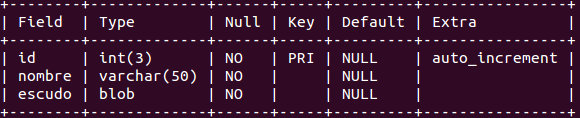
\includegraphics{images/tabla_equipos.png}
		\caption{Estructura de la tabla de equipos MySQL.}
	\end{figure}
	\item Tabla de rankings.
	\begin{figure}[H]
		\centering
		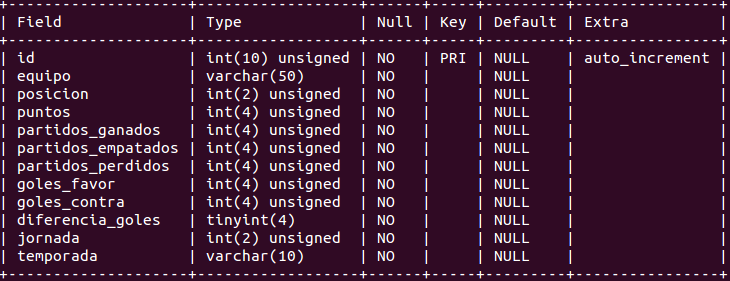
\includegraphics[scale=0.8]{images/tabla_rankings.png}
		\caption{Estructura de la tabla de rankings MySQL.}
	\end{figure}	
	\item Tabla de partidos.
	\begin{figure}[H]
		\centering
		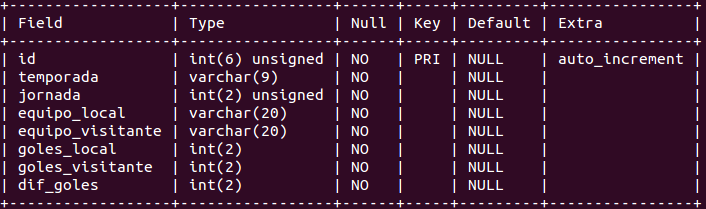
\includegraphics[scale=0.88]{images/tabla_partidos.png}
		\caption{Estructura de la tabla de partidos MySQL.}
	\end{figure}
\end{itemize}

\subsubsection{API REST}
REST (\textbf{RE}presentational \textbf{S}tate \textbf{T}ransfer) es un tipo de arquitectura de desarrollo web que se apoya totalmente en el estándar HTTP definida en el año 2000 por Roy Fielding (coautor también de la especificación HTTP). \\

Existen tres niveles de calidad a la hora de aplicar REST en el desarrollo de una API, que se recogen en el Modelo de Madurez de Richardson\cite{refapi1}\cite{refapi2}:
\begin{itemize}
	\item Nivel 0: consiste en el uso de HTTP como sistema de transporte sin usar otros mecanismos que permita la web.
	\item Nivel 1: vamos a trabajar con información que querremos consultar, modificar o borrar independientemente de su formato, es a lo que denominaremos ``recurso''. Estos recursos deben de tener una URL (Uniform Resource Locator) única que lo identifique y nos permita acceder a su ubicación.
	\item Nivel 2: consiste en la incorporación de los métodos HTTP (GET para consultar, POST para crear, PUT y PATCH para editar y DELETE para eliminar) así como los distintos códigos de estado que devuelve HTTP.
	\item Nivel 3: HATEOAS (Hypertext As The Engine Of Application State) consiste en conectar mediante hipervínculos las aplicaciones clientes con las APIs, permitiendo a dichos clientes despreocuparse por conocer de antemano del cómo acceder a los recursos.
\end{itemize}

\begin{figure}[H]
	\centering
	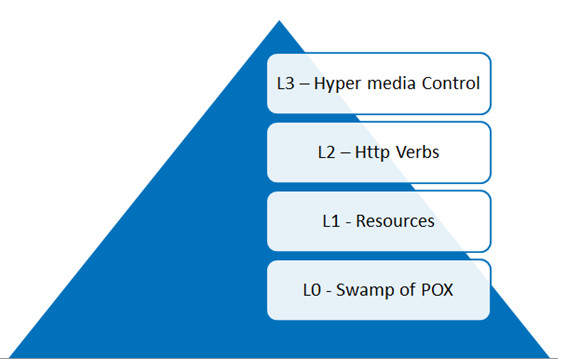
\includegraphics{images/apirest.png}
	\caption{Modelo de Madurez de Richardson.}
\end{figure}

La API implementada llega hasta el nivel 2 del Modelo de Madurez de Richardson. La herramienta que hemos empleado en su implementación es PHP con ayuda del micro framework Slim, que es de gran utilidad para la creación de APIs.\\

En \cite[Anexo A]{tfgjose} se pueden encontrar todos los métodos de la API Rest que se encontraban previamente implementados en la aplicación. Para el intercambio de información entre cliente y servidor usaremos el formato JSON por su simplicidad. \\

Al incluir el nuevo módulo de predicción hemos tenido que incorporar una nueva llamada a la API:
{\small \begin{center}
	\begin{tabular}{|c|c|}
	\hline URL  & /sport/:sportname/:league/prediction \\ 
	\hline Método & GET \\ 
	\hline Descripción & Devuelve la predicción para la próxima jornada de la liga :league del deporte :sportname\\ 
	\hline 
\end{tabular} 
\end{center}}

La llamada anterior devuelve un JSON que consta de 6 elementos, en orden:
\begin{enumerate}
	\item las probabilidades de resultados de los partidos calculadas por el modelo de interpolación,
	\item el ranking resultante usando el modelo de interpolación,
	\item las probabilidades de resultados de los partidos calculadas por el modelo de tendencias,
	\item el ranking resultante usando el modelo de tendencias,
	\item las probabilidades de resultados de los partidos calculadas por la combinación de los dos modelos, y
	\item el ranking resultante usando la combinación de los dos modelos.
\end{enumerate}

\ \\
Para obtenerlos se hace uso de funciones implementadas en distintos scripts PHP que realizan los cálculos matemáticos explicados en el capítulo 3 de esta memoria. \\

Para realizar la predicción aplicando el modelo de interpolación necesitamos obtener los umbrales que vamos a usar en los cálculos de las probabilidades. Para ello usaremos una clase Java que obtiene los umbrales desde la temporada que pongamos como inicio hasta la actual y los exporta como un archivo de texto.\\

Para realizar la predicción aplicando la combinación convexa de los dos modelos necesitamos ``entrenar'' sobre un histórico de datos y quedarnos con el valor de $\lambda$ que mejores resultados obtenga. Para ello usamos un script que prueba todos los valores de $\lambda$ desde $\lambda=0$ hasta $\lambda=1$ aumentando en cada paso $0.01$. Una vez obtenido el valor óptimo de $\lambda$ lo fijamos en el script que calcula las probabilidades.  

\subsection{Frontend}
El frontend consta de la aplicación AngularJS que será la encargada de hacer peticiones a la API REST y mostrar los resultados devueltos.\\

Tendremos que crear las vistas y controladores correspondientes al nuevo módulo de predicción añadido. En el controller se realizará la petición a la API REST y se guardará la respuesta obtenida en el scope para su posterior uso en el HTML correspondiente. También tendremos que modificar todas las demás vistas y controladores para poder acceder al nuevo módulo desde el resto de vistas ya existentes.\\

Todos los aspectos relacionados con las vistas con las que ya contaba la aplicación anteriormente se pueden encontrar en \cite[sección 3.4.1.]{tfgjose}.\\


\subsubsection{Vista del módulo de predicción}
En la figura \ref{fig:pprinc} se muestra la vista principal de la aplicación cada vez que la iniciamos. En la esquina superior derecha aparece el formulario desde el que podemos registrarnos o iniciar sesión para acceder al módulo de subir nuestros propios rankings. En el lateral izquierdo aparecerán todas las temporadas desde 1928/1929 hasta la más reciente, todos los equipos que han jugado alguna vez en Primera División y nuestro recién añadido módulo de predicción de resultados deportivos.\\

Cuando accedamos al módulo de predicción nos aparecerá una vista que consta de tres partes, cada una de ellas con dos tablas (las probabilidades de los resultados de los partidos de la próxima jornada y la predicción de la clasificación), que se corresponden respectivamente con cada uno de los tres modelos propuestos, el basado en la posición de los equipos (figura \ref{fig:pmod1}), el basado en la tendencia de los equipos en los últimos partidos (figura \ref{fig:pmod2}) y la combinación de ambos (figura \ref{fig:pmod3}).

\newpage

\begin{figure}[H]
	\centering
	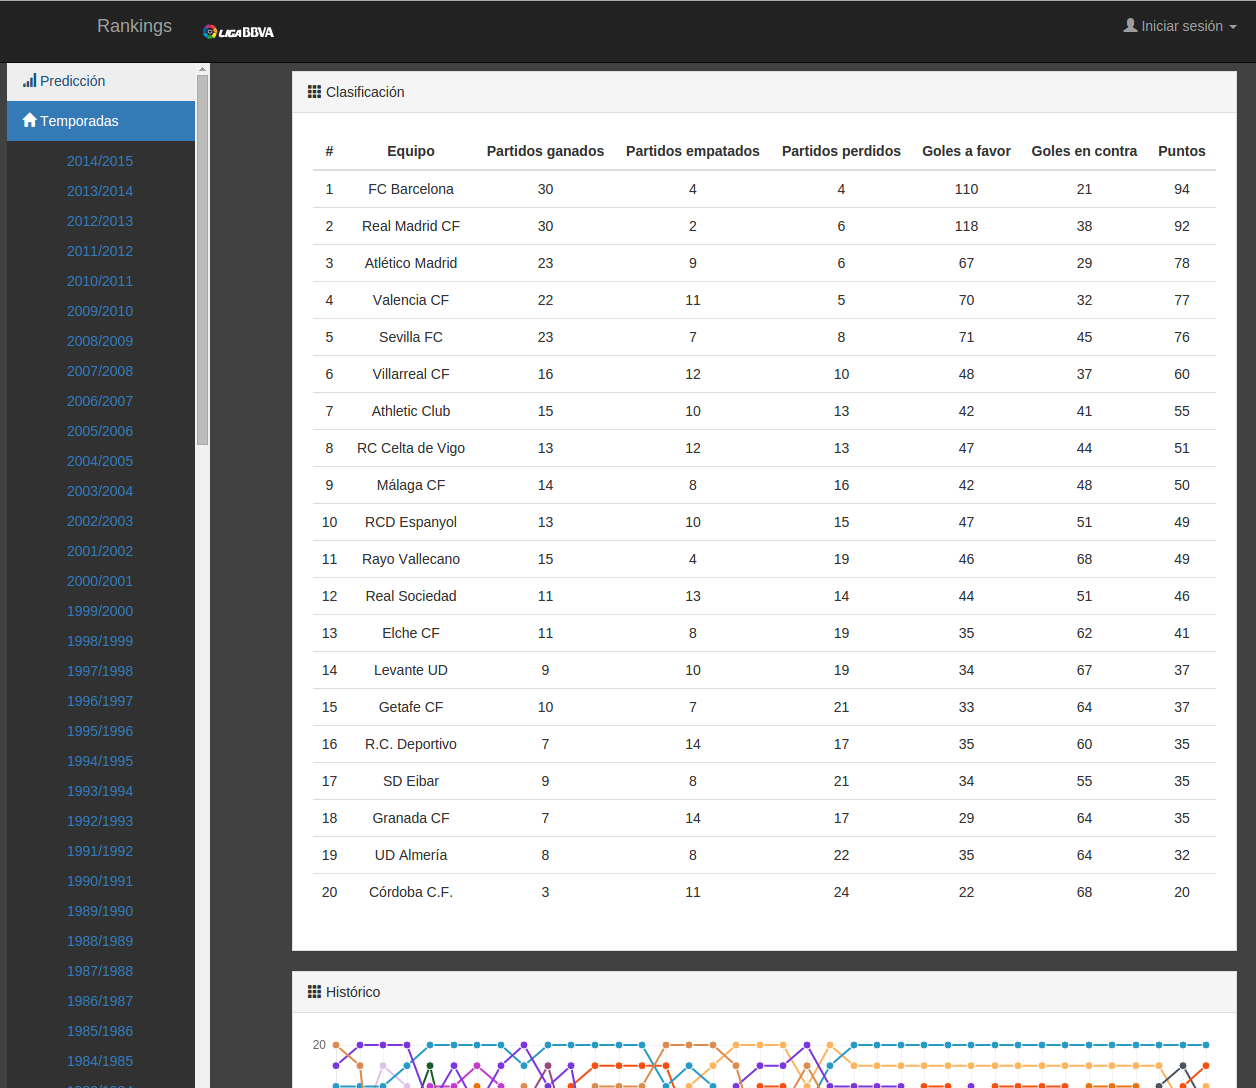
\includegraphics[scale=0.525]{images/pant_principal.png}
	\caption{Pantalla principal de la aplicación.} \label{fig:pprinc}
\end{figure}
\begin{figure}[H]
	\centering
	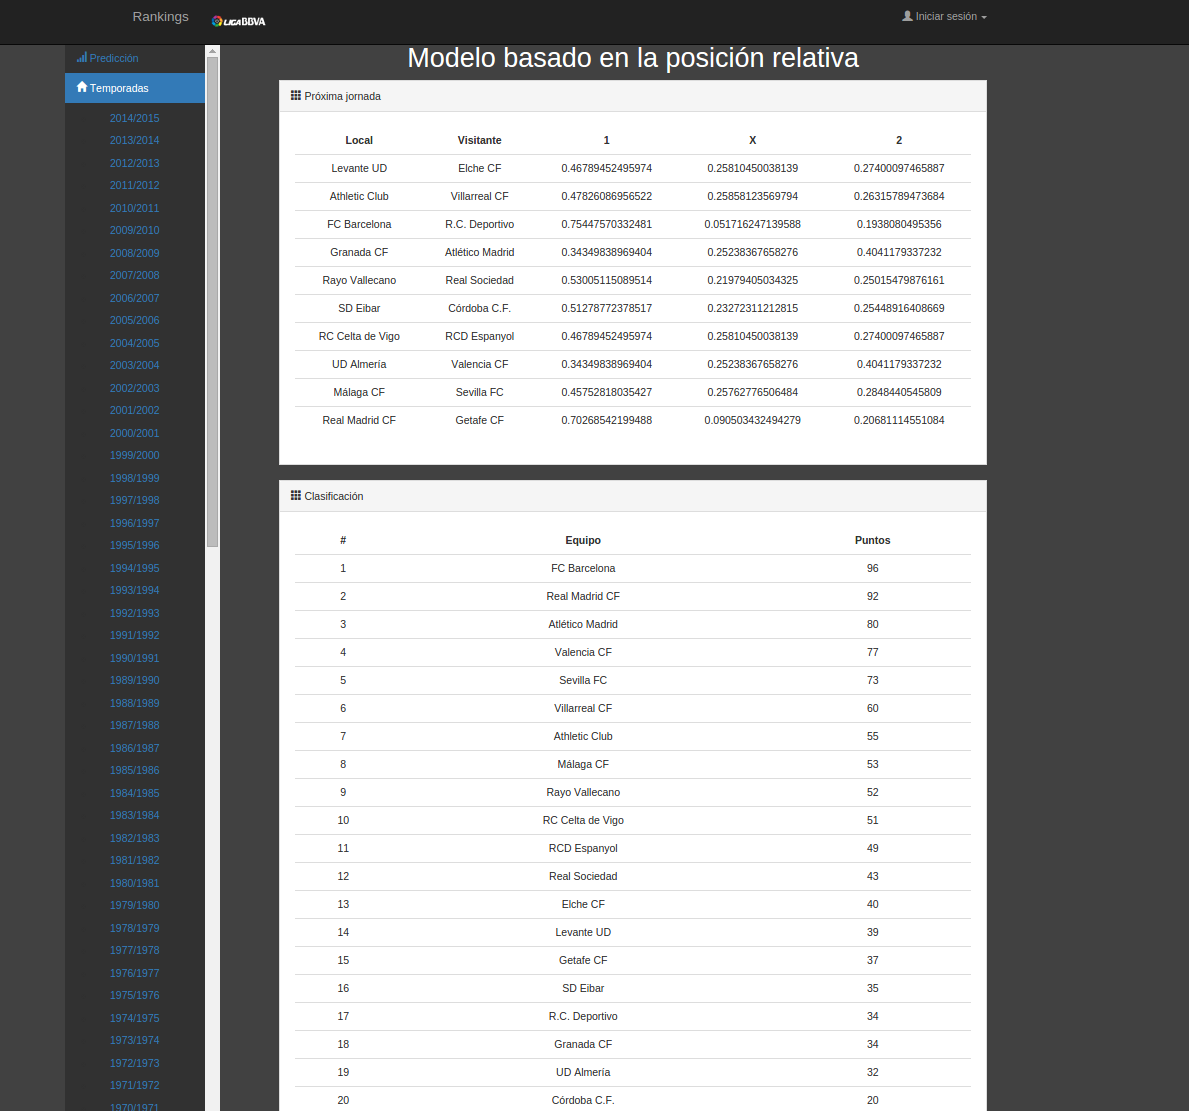
\includegraphics[scale=0.55]{images/pant_pred1.png}
	\caption{Vista del modulo de predicción(I).} \label{fig:pmod1}
\end{figure}
\begin{figure}[H]
	\centering
	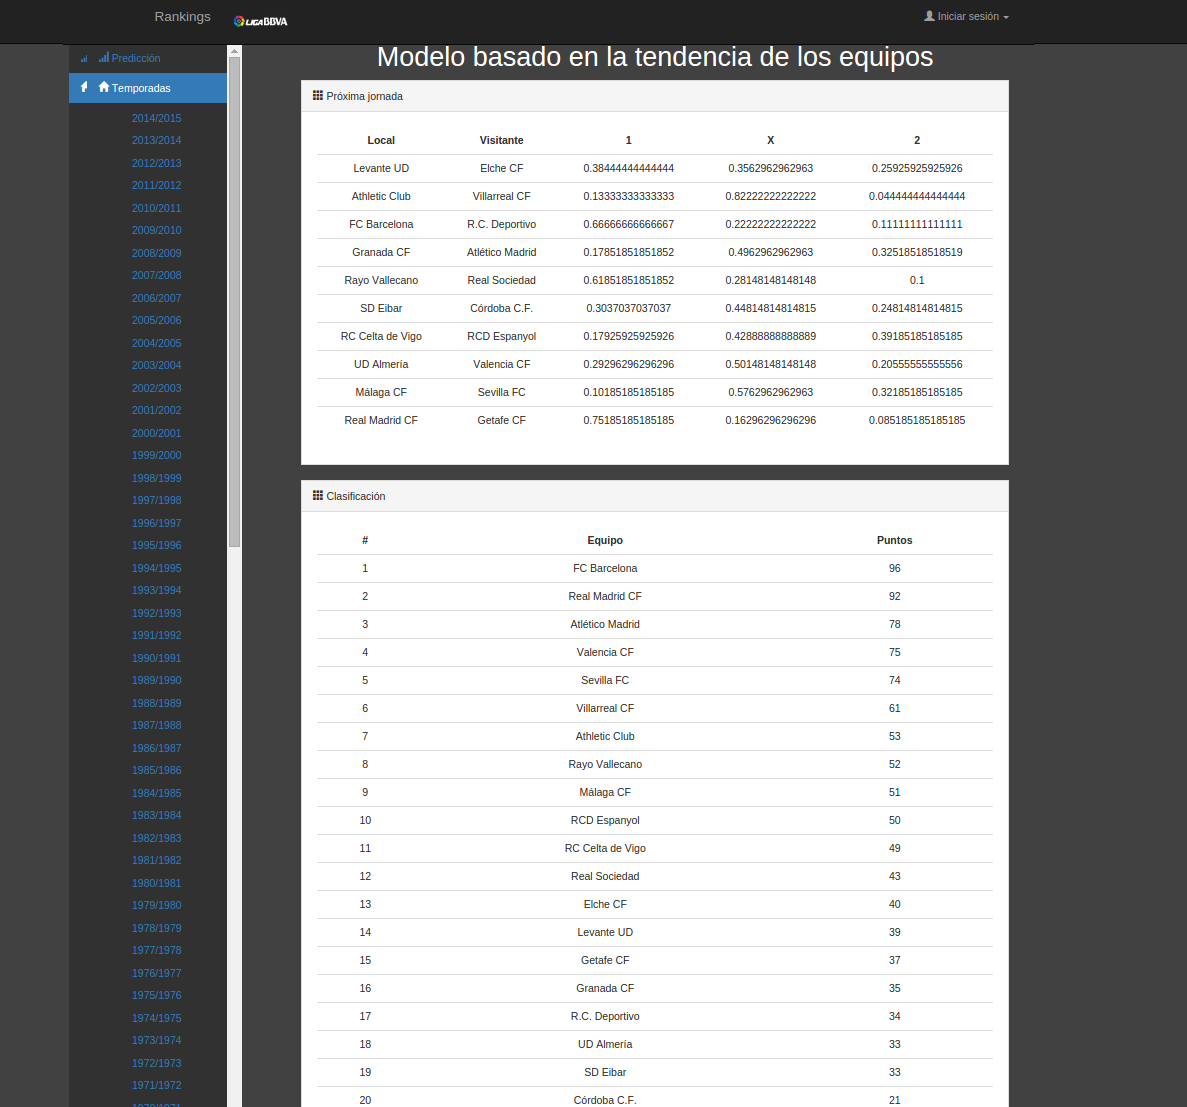
\includegraphics[scale=0.55]{images/pant_pred2.png}
	\caption{Vista del modulo de predicción(II).} \label{fig:pmod2}
\end{figure}
\begin{figure}[H]
	\centering
	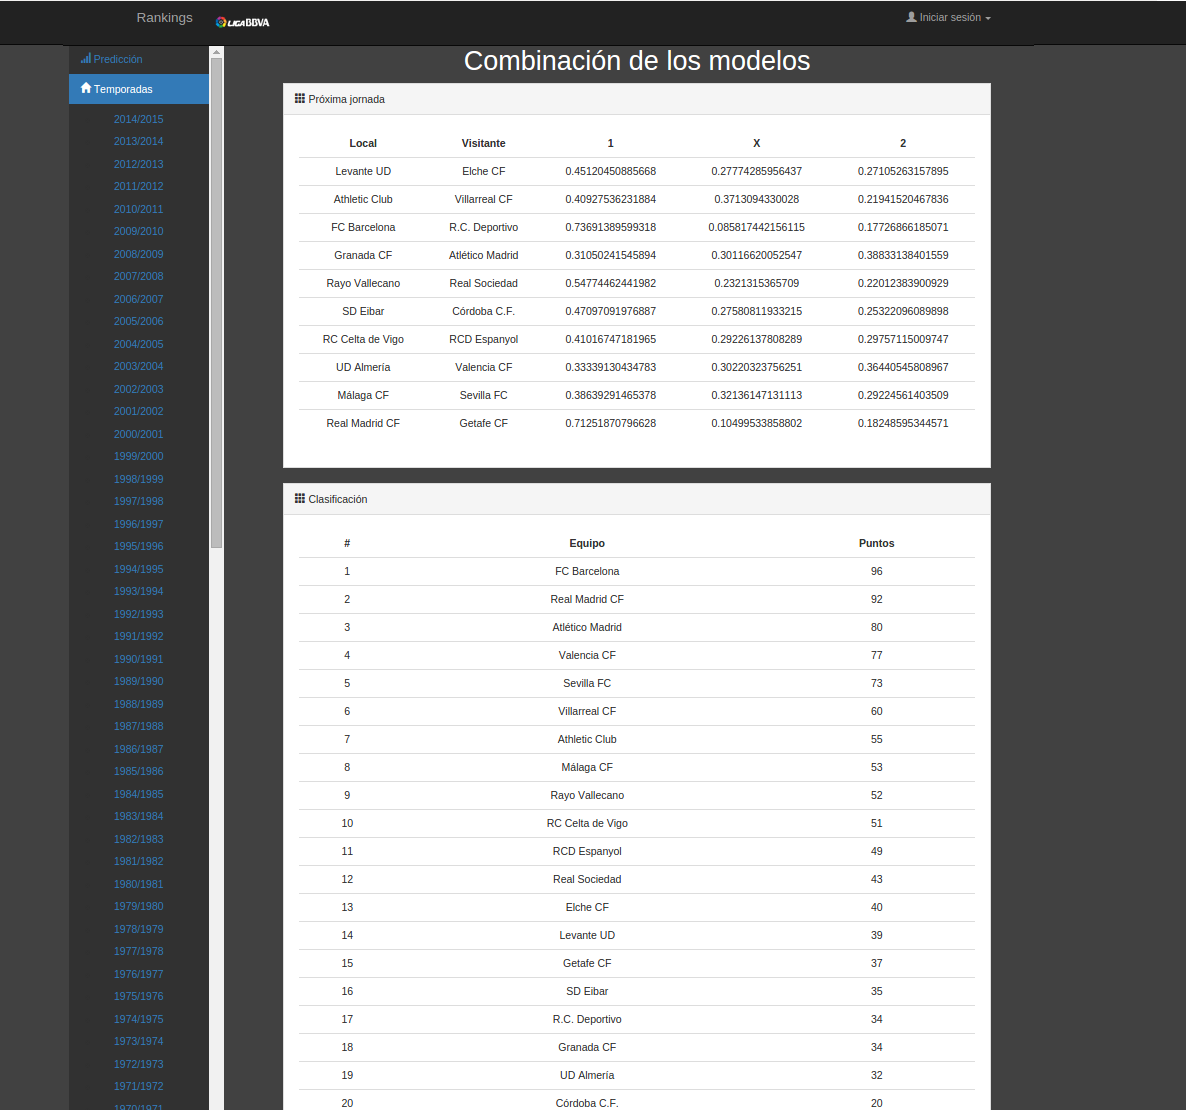
\includegraphics[scale=0.55]{images/pant_pred3.png}
	\caption{Vista del modulo de predicción(III).} \label{fig:pmod3}
\end{figure}